\documentclass[letterpaper]{article}
\usepackage{tabularx} % extra features for tabular environment
\usepackage{amsmath}  % improve math presentation
\usepackage{amsfonts} % Mathematics symbols
\usepackage{graphicx} % takes care of graphic including machinery
\usepackage[margin=1in,letterpaper]{geometry} % decreases margins
\usepackage{cite} % takes care of citations
\usepackage[final]{hyperref} % adds hyper links inside the generated pdf file
\hypersetup{
	colorlinks=true,       % false: boxed links; true: colored links
	linkcolor=blue,        % color of internal links
	citecolor=blue,        % color of links to bibliography
	filecolor=magenta,     % color of file links
	urlcolor=blue         
}
\usepackage{blindtext}
%++++++++++++++++++++++++++++++++++++++++

\begin{document}

\title{\vspace{-2.0cm}\textbf{Statistical Language Models}}
\author{Maneesh Kumar Singh \\ \small mksingh4@illinois.edu}
\date{\today}
\maketitle

\begin{abstract}
	In this technical review of Statistical Language Models, we first
provide brief introduction of language models and its two very popular
types: n-grams and neural language models. We compare the pros and cons
of these models and summarize our findings.
\end{abstract}

\section{Introduction}
Statistical language model is a probabilistic model for text data,
which defines distributions over sequences of words. Such model is 
often also called a generative model for text data because it can be
used for sampling sequences of words.

More formally, if we have some text $x^{(1)},...,x^{(T)}$, then the 
probability of this text according to the Language Model is
\begin{align}
	P(x^{(1)},...,x^{(T)}) &= P(x^{(1)}) \times P(x^{(2)}|x^{(1)}) \times ... \times P(x^{(T)}|x^{(T-1)},..,x^{(1)}) \\
	&= \prod_{t=1}^T P(x^{(t)}|x^{(t-1)},..,x^{(1)})
\end{align}

\section{n-gram Language Models}
An n-gram is a chunk of n consecutive words. Given text 
``The water is so transparent that'', its n-grams are
\begin{itemize}
	\setlength\itemsep{0em}
	\item unigrams: ``The'', ``water'', ``is'', ``so'', ``transparent'', "that''
	\item bigrams: ``The water'', ``water is'', ``is so'', ``so transparent'', ``transparent that''
	\item trigrams:``The water is'', ``water is so'', ``is so transparent'', ``so transparent that''
	\item 4-grams: ``The water is so'', ``water is so transparent'', ``is so transparent that''
\end{itemize} and so on.

The idea is to collect statistics about how frequent different n-grams are,
and use these to predict next words. In order to do so, we make a Markov
assumption: $x^{(t+1)}$ depends only on preceding n-1 words.
\begin{align}
	P(x^{(t+1)}|x^{(t)},...,x^{(1)}) &= P(x^{(t+1)}|x^{(t)},...,x^{(t-n+2)}) \label{eq:assumption} \\
	&= \frac{P(x^{(t+1)},x^{(t)},...,x^{(t-n+2)})}{P(x^{(t)},...,x^{(t-n+2)})} \label{eq:condprob}
\end{align}

To compute the probabilities mentioned above, the count of each
n-gram can be compared against the frequency of each word.
This is called an n-gram Language Model. For example, if the model
takes bi-grams, the frequency of each bi-gram, calculated via combining
a word with its previous word, would be divided by the frequency of
the corresponding uni-gram. Equations \ref{eq:bigram} and \ref{eq:trigram}
shows this relationship for bigram and trigram models.
\begin{align}
	p(w_2|w_1) &= \frac{count(w_1,w_2)}{count(w_1)} \label{eq:bigram} \\
	p(w_3|w_1,w_2) &= \frac{count(w_1,w_2,w_3)}{count(w_1,w_2)} \label{eq:trigram}
\end{align}

\subsection{Pros}
\begin{itemize}
	\item Really easy to build
	\item Can train on billions and billions of words
\end{itemize}

\subsection{Cons}
n-gram language model suffers from sparsity problem. Sparsity is used
to describe the situation of not observing enough data in corpus to
model language accurately. 

\begin{itemize}
	\item Note the numerator of Equation \ref{eq:trigram}. If $w_1$, $w_2$,
	and $w_3$ never appear in corpus together in the corpus, the probability of 
	w3 is 0. To solve this, a small $\delta$ can be added to the count of each 
	word in the vocabulary. This is called \textit{smoothing}.
	\item Consider the denominator of Equation \ref{eq:trigram}. 
	If $w_1$ and $w_2$ never occurred together in the corpus, then 
	no probability can be calculated for $w_3$.
	To solve this, we could condition on $w_2$ alone. This is called
	\textit{backoff}.
	\item Increasing $n$ makes sparsity problems worse. Typically, $n \leq 5$.
\end{itemize}

n-gram language model also suffers from storage problem.
\begin{itemize}
	\item As $n$ increases (or the corpus size increases), the model size increases
	as well.
\end{itemize}

\section{Window-based Neural Language Model}
Bengio et al introduced a Neural Probabilistic Language Model. It was
first large-scale deep learning model for natural language processing.
This model learns a \textit{distributed representation of words}, along
with the probability function for word sequences expressed in terms of
these representations. Figure \ref{fig:nplm} shows the corresponding
neural network architecture. The input word vectors are used by both
the hidden layer and output layer.

% In this model, the probabilistic prediction $P(x^{(t+1)}|x^{(t)},...,x^{(t-n+2)})$
% is obtained as follows. First each word 

\begin{figure}[ht]
	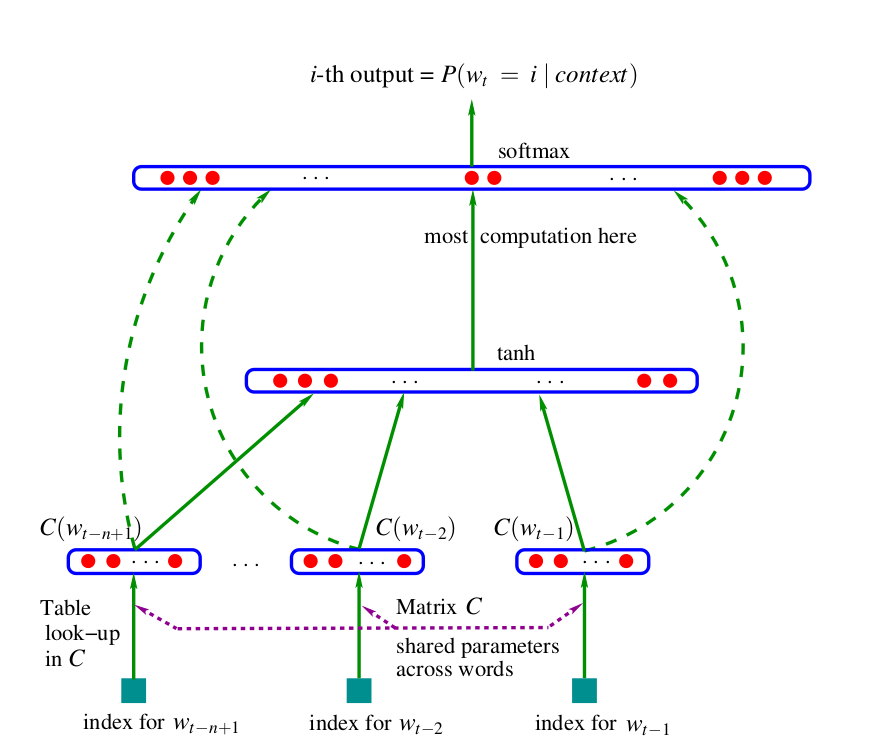
\includegraphics[scale=0.3]{images/Neural_Language_Model.png}
	\caption{The first deep neural network architecture model
	for NLP presented by Bengio et al.}
	\label{fig:nplm}
\end{figure}


Equation \ref{eq:nplm} represents Figure \ref{fig:nplm} and shows the
parameters of the $softmax()$ function, consisting of standard $tanh()$
function (i.e. the hidden layer) as well as the linear function, 
$W^{(3)}x + b^{(3)}$, that captures all the previous $n$ input word vectors.

A simplified version of this model can be seen in Figure
\ref{fig:nplmsimple}, where the blue layer represents
concatenated word embeddings for the input words:
$e = [e^{(1)};e^{(2)};e^{(3)};e^{(4)}]$, the red layer signifies
the hidden layer: $h = f(W_e + b_1)$, and the green output distribution
is a softmax over the vocabulary: $\hat{y} = softmax(Uh + b_2)$.


\begin{figure}
	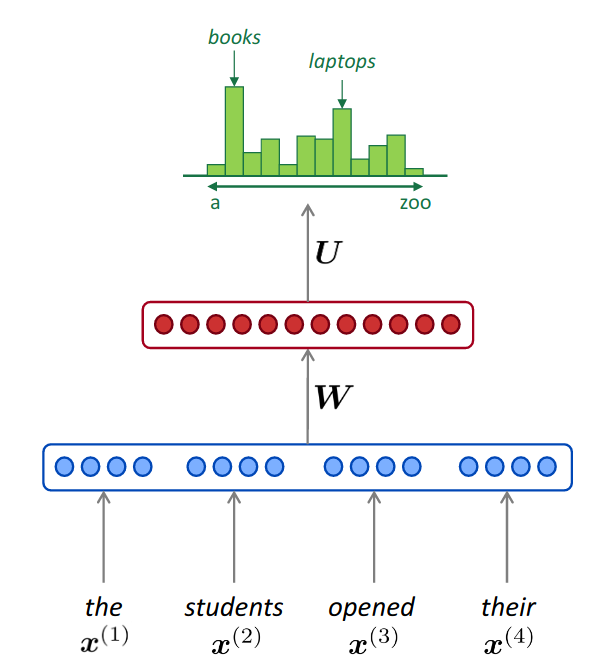
\includegraphics[scale=0.4]{images/Simplified_Neural_Language_Model.png}
	\caption{A simplified representation of Figure \ref{fig:nplm}}
	\label{fig:nplmsimple}
\end{figure}

\begin{align}
	\hat{y} &= softmax(W^{(2)}tanh(W^{(1)}x 
			+  b^{(1)}) + W^{(3)}x + b^{(3)}) \label{eq:nplm} \\
	\hat{y} &= softmax(Uh + b_2) \in \mathbb{R}^{|V|} \label{eq:nplmsimple} 
\end{align}


\subsection{Pros}
\begin{itemize}
	\item No sparsity problem
	\item Don't need to store all observed n-grams
\end{itemize}

\subsection{Cons}
\begin{itemize}
	\item Fixed window is too small
	\item Enlarging window enlarges $W$
	\item Window can never be large enough
	\item $x^{(1)}$ and $x^{(2)}$ are multiplied by completely different
	weights in $W$. No symmetry in how the inputs are processed.
\end{itemize}

\section{Recurrent Neural Networks (RNN)}
Unlike the conventional translation models, where only a finite
window of previous words would be considered for conditioning
the language model, Recurrent Neural Networks (RNN) are capable
of conditioning the model on all previous words in the corpus.

Figure \ref{fig:rnn} introduces RNN architecture where each
vertical rectangular box is a hidden layer at a time-step $t$.
Each such layer holds a number of neurons, each of which performs
a linear matrix operation on its inputs followed by a non-linear
operation (e.g. $tanh()$). At each time-step, there are two inputs
to the hidden layer: the output of previous layer $h_{t-1}$, and
the input at that time-step $x_t$. The former input is multiplied
by a weight matrix $W^{(hx)}$ to produce output features $h_t$,
which are multiplied with a weight matrix $W^{(S)}$ and run through
a softmax over the vocabulary to obtain a prediction output $\hat{y}$
of the next word(Equation \ref{eq:weight} and \ref{eq:sfmax}).

\begin{align}
	h_t &= \alpha(W^{(hh)}h_{t-1} + W^{(hx)}x_{[t]}) \label{eq:weight} \\
	\hat{y}_{t} &= softmax(W^{(S)}h_t) \label{eq:sfmax}
\end{align}

\begin{figure}[ht]
	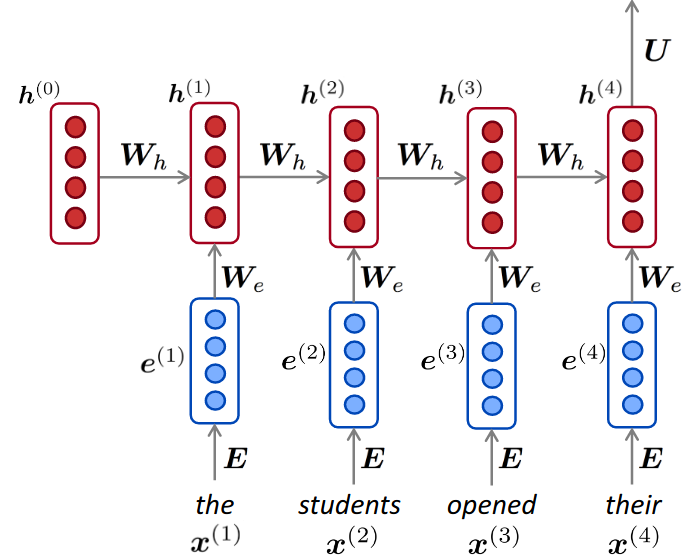
\includegraphics[scale=0.3]{images/RNN.png}
	\caption{An RNN Language Model}
	\label{fig:rnn}
\end{figure}



\subsection{Pros}
\begin{itemize}
	\item They can process input sequence of any length
	\item The model size does not increase for longer input sequence lengths
	\item Computation for step $t$ can (in theory) use information from many 
	steps back
	\item The same weights are applied to every time-step of the input, so
	there is symmetry in how inputs are processed
\end{itemize}

\subsection{Cons}
\begin{itemize}
	\item Computation is slow - because it is sequential, it cannot be
	parallelized
	\item In practice, it is difficult to access information from many steps
	back due to problems like vanishing and exploding gradients
\end{itemize}



\section{Summary}
In this review we compared n-grams, neural and its improvement RNN language model.
We noticed even though n-gram suffers from storage and sparsity problem. It's performance
is better than neural language models with comparable accuracy. Neural language model
provides better accuracy, but its accuracy is again restricted by window size. RNN overcomes
the issue with neural language model, but is slow and cannot access information from
many steps. Recently few models are developed over RNN which deals with performance and information
access problems e.g. Long short-term memory(LSTM) and Gated recurrent units (GRUs).

\begin{thebibliography}{9}
	\bibitem{iretrieval}
	ChengXiang Zhai and Sean Massung.
	\textit{Text Data Management and Analysis: A Practical Introduction to Information Retrieval and Text Mining}. 
	
	\bibitem{bengio} 
	Yoshua Bengio, Réjean Ducharme, Pascal Vincent and Christian Jauvin(2003).
	\href{https://www.jmlr.org/papers/volume3/bengio03a/bengio03a.pdf}{\textit{A Neural Probabilistic Language Model}}.
	Journal of Machine Learning Research, 3, 1137–1155.
	
	\bibitem{cs224n} 
	Stanford CS224n Lecture-6 Language Models and RNNS.
	\href{http://www.cs.umd.edu/class/fall2016/cmsc723/slides/slides_08.pdf}{Lecture Slides}.
	\href{http://web.stanford.edu/class/cs224n/readings/cs224n-2019-notes05-LM_RNN.pdf}{Lecture Notes}.
	\href{https://www.youtube.com/watch?v=iWea12EAu6U}{Youtube Video}.
\end{thebibliography}


\end{document}
